
\chapter{Estado del Arte}\label{chapter:introduction}

Actualmente existe una creciente preocupación por el cuidado animal donde la aparición de nuevas tendencias tecnológicas ha permitido el desarrollo de aplicaciones que facilitan no solo el cuidado de las mascotas por sus dueños, sino que hacen mucho más fácil el trabajo de las clínicas veterinarias como el de los profesionales de la salud.

Es así, como se puede observar un aumento de aplicaciones para Android dirigidas a establecimientos veterinarios que consiguen optimizar muchas de las tareas relacionadas con esta actividad permitiendo prestar un mejor servicio por parte de dichos clínicas veterinarios y a su vez ofrecerle suficiente información al dueño de la mascota de manera que pueda tomar la mejor decisión cuando se trata de vigilar la salud del animal y la elección del centro veterinario que mejor lo atienda.

En este capítulo se estudiará en que consisten las historias clínicas y que papel juegan dentro de la medicina veterinaria. Además, se analizarán algunas de las aplicaciones que en la actualidad tienen funcionalidades similares a las que se plantean en este documento para ser implementadas en el producto final. Así como las prestaciones de algunas de las aplicaciones encontradas que han sido desarrolladas en nuestro país en favor del bienestar animal. Luego de esto se estudian las posibilidades para la construcción del software en cuestión, decidiéndose una plataforma de desarrollo de aplicaciones móviles y un modelo de base de datos para almacenar los datos de manera local.\newpage


\section{La historia clínica en la medicina veterinaria}

La historia clínica (HC) es el documento que avala legalmente el trabajo del médico, pues en ella se expresan los resultados obtenidos en el diagnóstico clínico, y sirve de apoyo para el planeamiento, ejecución y control en cada caso, de las acciones destinadas a la recuperación y rehabilitación de la salud del paciente. Es un instrumento mediador a través del cual el médico elabora el diagnóstico, fundamenta el pronóstico, consigna el tratamiento y la evolución del paciente, siendo un documento único, integrado y acumulativo para cada paciente. La existencia de normas y leyes que hacen obligatorio su empleo, argumentan desde el punto de vista jurídico y normativo sus usos en lo asistencial, formativo y docente, científico e investigativo, evaluador de la calidad asistencial, administrativo y jurídico legal. De esta forma, la HC se convierte en el soporte escrito sobre el cual quedan las evidencias de la atención médica integrada que hacen todos los profesionales y técnicos de la salud partícipes en la misma \brackcite{odio2019historia}. 

El profesor cubano Llanio Navarro la considera como una guía metodológica para la identificación integral de los problemas de salud de cada paciente que establece todas sus necesidades. Es fundamental para analizar el proceso patológico del paciente y su evolución. A partir de lo expresado, toda la información que se obtiene con exactitud en la inspección médica debe ser registrada en un documento llamado HC \brackcite{cuenca2014historia}. 

Todos los datos registrados en este documento se obtienen realizando el método clínico, por las diferentes vías:
\begin{itemize}
\item	\textbf{ Anamnesis}: información que surge de la entrevista clínica proporcionada por el dueño del paciente. Es en esta sección donde se indica que ha ocurrido con el paciente, mencionado de forma ordenada los distintos síntomas y dolencias que la mascota ha presentado.
\item	\textbf{ Exploración física}: pruebas o exámenes complementarios realizados por el médico; juicios de valor que el propio médico extrae de documentos que él elabora para fundamentar un diagnóstico, prescribir el tratamiento y finalmente dejar constancia del curso de la enfermedad y el tratamiento instaurado.
\end{itemize}


Entre la información contenida en la historia clínica veterinaria se encuentran:
\begin{itemize}


\item \textbf{ Datos relativos al animal}: nombre y características físicas, fecha de nacimiento, sexo, etc. También en este punto se incluye la información relativa al propietario, datos de contacto, etc.
\item \textbf{ Datos proporcionados por el propietario de forma subjetiva}: a través de algunas preguntas, el personal veterinario anotará toda la información que proporcione el propietario, cómo qué le ocurre, desde cuándo, comportamientos extraños en el animal, síntomas, etc.
\item \textbf{Datos objetivos obtenidos de la exploración clínica}: el veterinario hará una exploración completa del animal para concretar la información recibida, y todo ello aparecerá también anotado en la historia clínica.
\item \textbf{Diagnóstico, pronóstico y tratamiento}: una vez recabados todos los datos, el veterinario tendrá que tomar nota del diagnóstico del animal, del pronóstico y del tratamiento a seguir. Del mismo modo, será necesario realizar revisiones para comprobar la efectividad del tratamiento, lo que también tendrá que aparecer dentro de la historia clínica del animal.
\end{itemize}

La HC es única para cada paciente, este último es sujeto de su propia investigación, la cual comienza con el diagnóstico de su enfermedad. Cabe agregar que por razones económicas y gerenciales la HC debe estar siempre disponible y facilitarse en los casos legalmente contemplados, resguardando la confidencialidad de los datos reflejados en ella. El acceso al expediente clínico sin autorización, en detrimento de un tercero, está catalogado como delito.

Se advierte que el redactar datos y argumentaciones en la historia clínica es una responsabilidad de los médicos (veterinarios) de atención, sobre la cual podrían, luego de un tiempo, sustentar sus propias evidencias defensivas ante posibles denuncias concernientes a su responsabilidad profesional. En Cuba la historia clínica es propiedad del hospital con un plazo de conservación y custodia de cinco años. Por lo cual, es conveniente recordar que cada actuación profesional que se realice debe ser datada con el tiempo y lugar donde se realiza, firmada, sellada con su cuño profesional y con las aclaraciones precisas sobre el acto ejercido   \brackcite{santana2016proposito}.

La HC puede presentarse en diferentes soportes: Papel que tradicionalmente ha sido manuscrito, teniendo inconvenientes para la legibilidad de la caligrafía por el volumen de espacio que ocupa y el deterioro con el paso del tiempo, videos, fotografías, estudios radiológicos y soporte informático. En los nuevos centros de atención médica y veterinaria las historias clínicas están informatizadas, mediante complejos sistemas informáticos \brackcite{garcia2006historia}.

La sustitución de la HC tradicional (en soporte papel) por la HCI responde a varias necesidades \brackcite{rueda2006historia}:  

\begin{enumerate}
	\item Dar cumplimiento a las características y objetivos del documento HC en cuanto a los requerimientos del equipo sanitario, manteniendo la confidencialidad.  
	
	\item Resolver los dos problemas clásicos de los archivos de HC el almacenamiento de grandes volúmenes documentales y la seguridad frente a los riesgos de pérdida y de deterioro.  
	
	\item Permitir la transferencia rápida de la información sanitaria existente de un paciente a puntos lejanos, garantizando que cada paciente solo tenga un único expediente y este pueda ser consultado simultáneamente en distintos lugares.  
	
	\item Soportar las decisiones médico-asistenciales, mediante la interacción con bases de datos, que permitan una rápida consulta de las mejores prácticas, los protocolos de manejo y las evidencias reconocidas.  
	
	\item Poner a disposición de los educadores, investigadores y de los planificadores sanitarios esta información, en forma eficiente. 
\end{enumerate}

La calidad en su confección está condicionada por muchos factores. Por un lado, está el nivel de exigencia en las instituciones; por otro, el nivel de aprendizaje de los que la confeccionan. Los problemas que puedan suscitar en su confección, pueden ser atribuidos al desconocimiento, beneficios o perjuicios derivados de un contenido incompleto  \brackcite{garcia2006historia}.

En la figura \ref{HCIvsHC} se resumen las diferentes características de la HC tradicional y la HCI a través de una comparación de sus fortalezas y debilidades.


\begin{center}
	\begin{figure}
		\caption{Diferencias entre la HCI y la HC tradicional. }
		\label{HCIvsHC}
		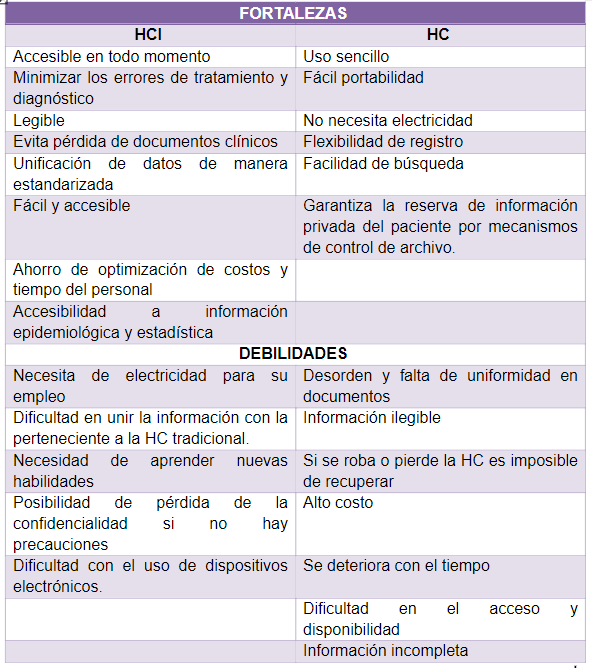
\includegraphics[]{MainMatter/HCIvsHC.PNG}
	\end{figure}
\end{center}


\subsection{Conclusiones}\label{chapter:introduction}


Las ciencias informáticas y bibliográficas han constituido un aporte significativo para el diseño y operación de los sistemas de información del sector sanitario, en especial de la HCI, la cual ha sido aplicada a la medicina veterinaria.

La motivación, y capacitación del personal sanitario, el uso de las herramientas informáticas y de comunicación, y la toma de decisiones basada en evidencias demostrables, se convierten en la piedra angular de los servicios de atención veterinaria.

Por ende, la historia clínica veterinaria constituye un documento único confidencial e individual, en el cual queda plasmado el pronóstico, tratamiento y la evolución del paciente, de ahí la importancia de su correcta confección. 
	

\newpage
\section{Aplicaciones desarrolladas en Cuba en favor del Bienestar Animal}\label{chapter:introduction}

\subsection{Web del Registro Cubano de Mascotas (RCM)}\label{chapter:introduction}


%\begin{figure}[h!]
%\begin{center}
%
\includegraphics[scale=0.4]{Graphics/images/LogodelRegistroCubanodeMascotas.jpg}
%\caption{Logo del Registro Cubano de Mascotas}
%\label{fig:rcm}

%\end{center}
%\end{figure}


Luego de más de 30 años de lucha finalmente Cuba aprueba un Proyecto de Ley sobre protección animal que busca defender los derechos de animales silvestres, de granja y de compañía. Los animales de granja y silvestres tienen derechos y una connotación legal y ética, pero no social. En cambio, los de compañía si pueden y deben entrar en este grupo por su vinculación estrecha al dueño, su familia y el entorno comunitario. Desde esta perspectiva se hace obligatorio que la mascota sea identificada oficialmente y cambiar su estatus de objeto a sujeto. En una reunión efectuada en marzo de 2006 en el Consejo Científico Veterinario de la Habana algunos médicos, técnicos y estudiantes veterinarios abogaron por realizar un estudio para un registro de las mascotas a través de una intranet del Instituto de Medicina Veterinaria. Su objetivo era poder acceder a los datos de las mascotas desde cualquier lugar del país.

Con este enfoque se crea la \textbf{web del Registro Cubano de Mascotas}\brackcite{insReg}, un espacio digital que brinda identificación, respaldo en el cuidado, protección y tenencia responsable de los animales de compañía. Como una de las particularidades se destaca la posibilidad de obtener un documento de identidad, totalmente gratuito; que llevará en él todos los datos de los animales que se inscriben y las de su persona responsable. Este es un proceso sencillo e intuitivo en el que se deben realizar los pasos mostrados a continuación:

\begin{itemize}
\item Acceder a través del teléfono celular o una computadora al sitio www.mascotascuba.com
\item Rellenar los datos solicitados como nombre de la mascota, fecha de su nacimiento, sexo, raza, foto, dirección.
\item Ingresar el correo electrónico o teléfono del tutor de la mascota.
\end{itemize}

Hasta agosto de 2021, estaban oficialmente registrados en la plataforma alrededor de 21 000 animales. De ellos, el $60 \%$ eran perros, $30 \%$ gatos, $7 \%$ aves y un $3 \%$ de roedores, reptiles, equinos, bovinos, porcinos, y otras especies.

\subsection{BACuba}\label{chapter:introduction}

%\begin{figure}[h!]
%\begin{center}
%
\includegraphics[scale=0.09]{Graphics/images/LogodeBienestarAnimalenCuba.png}
%\caption{Logo de Bienestar Animal en Cuba}
%\label{fig:bac}

%\end{center}
%\end{figure}

\textbf{ BACuba}\brackcite{apMov} \brackcite{cubDis} es una aplicación para teléfonos móviles que tiene como fin lograr el bienestar animal y sensibilizar a las personas para la protección de estos seres vivos. Dicha aplicación es una iniciativa de la organización \textbf{Bienestar Animal Cuba}\brackcite{pOBAC}, la mayor red de voluntarios para la protección animal. Fue lanzada desde el pasado 19 de enero de 2022, y se basa en el principio que rige la organización: rescatar animales abandonados y brindarles todos los cuidados. También buscan promover campañas, actividades, ferias y spots para garantizar el bienestar animal. Esta novedosa aplicación posee varias utilidades separadas en varias secciones:

\begin{itemize}
\item \textbf {Adoptar}: En este panel se muestran todos los datos (nombre, edad, sexo, raza) y con una foto incluida de los animales que están en adopción, ya sea perros, gatos u otros.
\item \textbf{ Reportes}: Esta es una de las secciones más humanas, ya que los usuarios podrán reportar desapariciones de mascotas, acciones de maltrato animal, atropellos, abandonos, animales en estado de vulnerabilidad. Pueden hacerlo desde cualquier parte del país y con estas denuncias los voluntarios de las distintas redes de ayuda animal o cualquier persona sensibilizada tomarán cartas en el asunto.
\item \textbf{Cuidados}: En este apartado se brindan informaciones de mucha ayuda para los dueños de mascotas y que son útiles para todas las provincias y municipios del país. Por ejemplo, una lista con direcciones y teléfonos de las principales clínicas veterinarias, tiendas de accesorios y medicinas para sus mascotas, y algunos artículos de interés para aumentar la cultura del cuidado animal.
\item \textbf{Noticias}: Aquí te podrás enterar de eventos relevantes como ferias de adopciones a lo largo de toda Cuba, donaciones y otras actividades en las que quizás te interese participar.
\item \textbf{Mis Mascotas}: En este apartado podrás registrar a tus animales con sus nombres, fecha de nacimiento, y todos los datos de su carnet de identidad, en el caso de poseer uno. En esta base de datos podrás incluir, además, un registro con los días de vacunación y desparasitación, a modo de recordatorio.
\end{itemize}

Información general de BACuba:


\begin{itemize}
\item Funciona con los datos móviles activados o por medio de servicio Wifi.
\item Está diseñada únicamente para dispositivos móviles, con un tamaño de 12.60 MB y requiere una versión de Android 5.0 o versiones superiores.
\item Es útil para cualquier lugar del país.
\item Puede ser descargada, libre de costo, de la plataforma APKLIS.
\item Tiene un diseño sencillo pero atractivo, y cumple con su función de informar, orientar, educar y ayudar en cuanto a materia de protección animal.
\end{itemize}

\section{Aplicaciones móviles que gestionan Historias Clínicas Veterinarias}\label{chapter:introduction}

\subsection{Dog Health}\label{chapter:introduction}

%\begin{figure}[h!]
%\begin{center}
%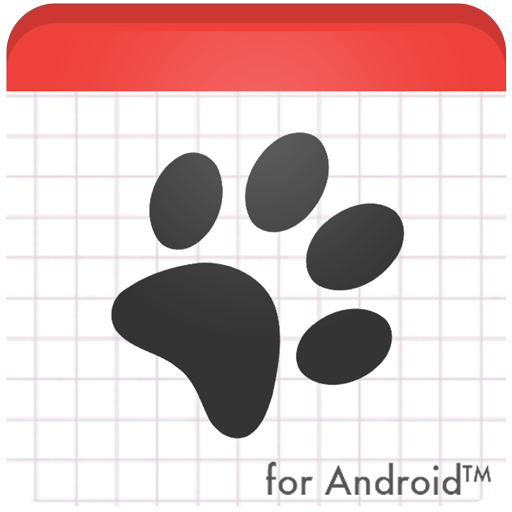
\includegraphics[scale=0.12]{Graphics/images/LogodeDogHealth.png}
%\caption{Logo de Dog Health}
%\label{fig:dh}

%\end{center}
%\end{figure}


\textbf{Dog Health}\brackcite{dogHe} es una aplicación totalmente gratuita para móviles y tablets, fue creada por un comunicador italiano, por lo que está solo disponible en el idioma inglés. Creada para llevar el registro veterinario de nuestras mascotas en Android. Dentro de sus principales prestaciones se encuentran:

\begin{itemize}


\item	Guardar los datos personales de las mascotas como su nombre, peso, fecha de nacimiento, número de chip, entre otros.
\item	Hacer un seguimiento de anteriores visitas al veterinario.
\item	Administrar a los veterinarios.
\item	Hacer un seguimiento de las vacunas.
\item	Recordatorios de citas y visitas.
\item	Memorizar todas las administraciones de medicamentos realizadas y por realizar.
\item Buscar y contactar con el veterinario más cercano.
\item	Añadir múltiples mascotas.
\item	Realizar backups y restaurarlos.
\item	Guardar la evolución del peso y altura de las mascotas de forma continuada.

\end{itemize}


\subsection{Pet Soft}\label{chapter:introduction}

%\begin{figure}[h!]
%\begin{center}
%
\includegraphics[scale=0.5]{Graphics/images/LogodePetSoft.png}
%\caption{Logo de Pet Soft}
%\label{fig:dh}

%\end{center}
%\end{figure}


\textbf{ Pet Soft}\brackcite{sofVet} \brackcite{petSo} es una plataforma para veterinarias y dueños de mascotas creada para almacenar y gestionar agendamientos con todo lo relacionado del paciente estableciendo citas, vacunas y todo tipo de información detallada con el fin de contar con un completo historial médico que le permita no solo al profesional veterinario, sino a los dueños de las mascotas acceder de manera segura a la información completa del animal. Esta plataforma es completamente web y la aplicación se puede descargar desde cualquier dispositivo con sistema operativo Android o IOS.

Como ventaja para el usuario sea médico o dueño de la mascota conseguirá descargar la aplicación de forma intuitiva donde podrá ingresar toda la información requerida y vital para los pacientes. Su fortaleza radica en la fácil visualización y datos de carga que aseguran una experiencia agradable para sus usuarios. Con la implementación del software los usuarios pueden gestionar de forma segura y sencilla todo lo relacionado con las mascotas y acceder a la ubicación de la red más completa de veterinarias. La información de cada mascota, se alberga en la web, de modo que, en cada centro veterinario, se podrá descargar, sin necesidad de que se tengan que volver a registrar los datos en el sistema. Dentro de sus principales beneficios se encuentran:

Beneficios para veterinarias:
\begin{itemize}


\item	Consultas y servicios: crear consultas y servicios; todo bajo control del software.
\item	Tarifas y bonos: manejar tus propias tarifas, generar bonos promocionales.
\item	Citas y alarmas: notificaciones para las citas programadas o crear una directamente.
\item	Veterinarias en red: consultar la historia clínica de la mascota si ha estado en otra veterinaria.
\item	Médicos veterinarios: crear usuarios especializados para tu veterinaria.

\end{itemize}

Beneficios para tu mascota:
\begin{itemize}


\item	Datos básicos: registrar todas las mascotas.
\item	Historia clínica: llevar el historial de las consultas de tus mascotas directamente de las veterinarias.
\item	Citas: notificaciones para las citas programadas o crear una directamente.
\item	Veterinarias: un mapa para buscar la veterinaria más cercana.
\item	Carné: llevar en la app el carnet de vacunación de tus mascotas.
\end{itemize}


\subsection{Petmeddata}\label{chapter:introduction}


\textbf{Petmeddata} \brackcite{petMed}\brackcite{petMed2} es un sistema electrónico seguro para almacenar el historial médico de todas las mascotas en un solo sitio. Creado en Finlandia a finales de 2018, facilita el tratamiento integral de los animales ya que muestra instrucciones de alta, medicamentos y valores de laboratorio en orden cronológico. Los problemas de seguridad se han considerado cuidadosamente. El dueño del animal decide quién puede ver la información de la mascota. Si el propietario comparte el perfil con una nueva clínica, esta puede ver las secciones más importantes del historial clínico en el historial del paciente. El personal de la clínica también ve las entradas, textos e imágenes del propietario. Nadie puede ver el precio y la información de pago, ni las notas de la clínica de animales. El nombre del animal o el microchip nunca aparecerán en ninguna parte. Para dueños de animales y clínicas de animales, el sistema es gratuito. A los socios se les cobra una tarifa por prestar sus servicios en el sistema.
“Al utilizar $Petmeddata$, el dueño siempre tiene consigo el historial médico de la mascota, incluso si va a una nueva clínica. Y el veterinario podrá leer en un formato fácil de leer lo que se le ha hecho al animal en el pasado. No hay necesidad de llevar papeles escritos a mano o impresos”, dice la Gerente de Proyecto Eva Kaisti.

Entre sus principales características se encuentran:
\begin{itemize}


\item	Fácil acceso online a todos los datos sanitarios de las mascotas; crea el perfil médico para cada uno de tus animales y contrólalos desde un solo sitio
\item	Veterinarios y otros expertos envían los datos médicos oficiales al perfil del animal.
\item	Posibilidad de añadir tus propios documentos y notas.
\item	Funciona por conexión a internet desde un teléfono móvil, tablet u ordenador.
\item	Sitio seguro; no almacena información personal tuya, sólo la información médica de tus mascotas.
\item	Posibilidad de compartir el perfil de las mascotas con un profesional del cuidado de los animales, como un veterinario, un amigo, guardería para mascotas, etc.
\end{itemize}


\subsection{VitusVet}\label{chapter:introduction}

\textbf{VitusVet} \brackcite{vitPet} es un $software$ de administración de prácticas veterinarias que permite a veterinarios y clínicas manejar el flujo de trabajo, comunicaciones con clientes, pagos, historias clínicas, horarios de consultas, entre otros. Permite el envío y recibimiento de texto, imágenes y actualizaciones en tiempo real.

Usando aplicaciones móviles de $VitusVet$ múltiples veterinarios pueden compartir historias clínicas de mascotas con clientes y hacer recordatorios sobre encuentros futuros. La plataforma $VitusPay$ permite a los dueños de mascota realizar pagos mensuales a través de tarjetas de crédito. Los clientes pueden pedir consultas con los veterinarios a través de mensajes de texto, emails, plataformas de redes sociales y aplicaciones móviles. El $software$ permite a veterinarios configurar y automatizar respuestas basándose en el personal disponible, horario de trabajo, días feriados y enviar recordatorios a través de postales personalizadas. 





\subsection{Conclusiones de las aplicaciones presentadas}\label{chapter:introduction}

En esta sección se analizaron aplicaciones con similitudes a la que se plantea como finalidad en este documento. Todo esto con el objetivo de adoptar las ideas de la competencia o mejorarlas dependiendo del caso, sobre este tema se puede afirmar lo siguiente:

\begin{enumerate}


\item	En general las herramientas en esta sección permiten la creación y el manejo de las historias clínicas digitales para nuestras mascotas, pero como se observó en cada caso estas no brindan la posibilidad para exportar de manera offline\footnote{La tranferencia de datos offline en $Android$ refiere a una forma de enviar datos de forma inalámbrica sin necesidad de conexión a Internet, existen varias tecnologías que permiten este tipo de transferencia como $Wifi$ $Direct$, $Bluetooth$, $SIP$, etc.} \brackcite{offDT} los datos de las mascotas que queramos compartir con otro usuario. Entre los objetivos de este trabajo está la mejora de este aspecto.



\item	Pocas de estas aplicaciones permiten al usuario consultar los datos de sus mascotas sin la necesidad de una conexión a Internet, aspecto que goza de gran peso entre los principales objetivos de este trabajo.
\item	Las herramientas para el manejo de las historias clínicas desde un dispositivo móvil, permiten a los usuarios ya sean médicos veterinarios o dueños y encargados de las mascotas acceder de manera sencilla y segura a toda la información referente al estado de salud, seguimiento, y cuidado del animal.
\item	Luego de analizar las aplicaciones anteriores se concluye como necesario el diseño de una aplicación que si cumpla con los requerimientos expuestos en este documento, porque en general estas aplicaciones no permiten el trabajo con historias clínicas animales de manera offline, aspecto de vital importancia debido a las limitaciones de la conexión a Internet que presenta nuestro país.
\end{enumerate}

\section{Tecnologías para el desarrollo de aplicaciones móviles}\label{chapter:introduction}

\subsection{Programación Nativa de Android : Java y Kotlin}\label{chapter:introduction}

El desarrollo de aplicaciones nativas es una opción increíble para ofrecer a los usuarios la experiencia más satisfactoria en términos de la sensación y la apariencia de su aplicación. 



\subsection{React Native}\label{chapter:introduction}



%\begin{figure}[h!]
%\begin{center}
%
\includegraphics[scale=0.5]{Graphics/images/LogodeReactNative.jpg}
%\caption{Logo de React Native}
%\label{fig:dh}

%\end{center}
%\end{figure}


\textbf{React Native}\brackcite{reaNative} es un framework que permite construir aplicaciones móviles nativas, para iOS y Android (así como también para Android TV, macOS, tvOS, Windows y UWP\footnote{Universal Windows Platform}  , aunque nos enfocaremos en los dos gigantes de la telefonía móvil), utilizando solamente JavaScript y React.

Utiliza el mismo diseño que React.js, permitiendo usar elementos de interfaz de usuario móvil. A pesar de que React.js y React Native usen la misma estructura de código, no sirven para lo mismo, mientras React.js es utilizado para hacer páginas web y trabaja con elementos del virtual DOM, por el otro lado React Native utiliza elementos nativos de interfaz de usuario de Android y iOS (entre otras) para crear aplicaciones para ambas plataformas.

Habiendo mencionado la UI, React Native usa el mismo paradigma fundamental de construcción de bloques para la interfaz de usuario que las aplicaciones nativas puras de Android e iOS (a los que React Native denomina Componentes), pero gestiona la interacción entre los mismos utilizando las capacidades de JavaScript y React.

Similar a React para web, en este caso las aplicaciones están escritas usando una mezcla de JavaScript y marcado XML, conocido como JSX\footnote{JavaScript Syntax Extension y ocasionalmente mencionado como JavaScript XML} . Luego, detrás del telón, el conocido \textbf{bridge} o puente de React Native invoca las APIs de renderizado nativas en Objective-C (para iOS) o Java (para Android). React Native también expone interfaces JavaScript para las API de la plataforma, por lo que sus aplicaciones pueden acceder a sensores y funciones de la plataforma como la cámara del teléfono o la ubicación del usuario.

React Native surgido por la necesidad de una solución nativa para los problemas que presentaba el uso de HTML5 en la versión móvil de Facebook, que resultó en una aplicación inestable y con poca fluidez. La idea surge a partir de Jordan Walke, ingeniero de software de Facebook, que encontró una forma de generar elementos de interfaz de usuario para iOS a partir de un hilo de JavaScript en segundo plano, lo que sentó las bases de lo que sería React para la web. Esto unido al interés de la compañía llevó a que meses más tarde Facebook lanzara la primera versión de React.js, y Christopher Chedeau\footnote{También conocido como Vjeux, es un ingeniero front-end en Facebook que se graduó de EPITA (la primera escuela de ingenieros especializada en informática de París)} , durante una charla técnica explicara, que Facebook ya estaba usando React Native en producción para su aplicación de grupo y su aplicación de administrador de anuncios.

Ventajas
\begin{enumerate}

\item	Traduce su marcado a elementos de UI nativos reales, además, React funciona por separado del hilo principal de la interfaz de usuario, por lo que su aplicación puede mantener un alto rendimiento sin sacrificar la capacidad.
\item	Para los desarrolladores acostumbrados a trabajar en la Web con React.js, significa que pueden desarrollar aplicaciones móviles con el rendimiento y la apariencia de una aplicación nativa, mientras usan herramientas familiares.
\item	Una comunidad sólida, hay miles de colaboradores que actualizan constantemente la biblioteca.
\item	Permite optimizar las aplicaciones nativas por separado escribiendo código específico de cada plataforma y usándolo desde JavaScript.
\item	Mejora la experiencia de desarrollo gracias a su Hot Reload o recarga en caliente, que permite a los desarrolladores visualizar cambios efectuados en la aplicación de inmediato, sin necesidad de re-compilar todo el proyecto.
\item	Alta fiabilidad al estar respaldada por Facebook, siendo usada como herramienta de desarrollo por grandes empresas como Instagram, Microsoft, Pinterest y Walmart.
\end{enumerate}

Desventajas
\begin{enumerate}



\item	La navegación integrada en React Native no es perfecta y no es comparable a la navegación nativa.
\item	Tiene dificultades para crear transiciones y animaciones complejas.
\item	Debido a que React Native es una abstracción sobre las API existentes de Android y iOS, usualmente cuando hay nuevas versiones puede ser que esa funcionalidad tarde un poco en llegar a la plataforma aunque siempre llega.
\item La documentación es deficiente para algunos casos, producto a la misma velocidad con que se realizan actualizaciones, muchos colaboradores no consideran necesaria su documentación sobre la marcha.
\end{enumerate}



\subsection{Xamarin}\label{chapter:introduction}

\textbf{Xamarin} \brackcite{xama} es un kit de herramientas de desarrollo de aplicaciones multiplataforma que nos permite producir aplicaciones nativas de $Android$, $iOS$, $tvOS$, $watchOS$, $macOS$ y $Windows$ con $UI$ unificadas, siendo parte en la actualidad de la plataforma de desarrollo $.NET$  \footnote{$.NET$ es una plataforma de desarrollo compuesta por herramientas, lenguajes de programación y bibliotecas para crear muchos tipos diferentes de aplicaciones.} \brackcite{net}. Fue en sus inicios construida como herramienta por los desarrolladores de Mono \footnote{Mono es una plataforma de desarrollo de código abierto basada en .NET Framework, dirigida por Miguel de Icaza y presentada por primera vez en 2001}  y siendo fundada como compañía homónima el 16 de mayo del 2011, para ser adquirida en el 2016 por Microsoft.
Fue para cuando Microsoft adaptó el $Kit$ de Desarrollo de Software ($SDK$) \footnote{Un $kit$ de desarrollo de software ($SDK$) es un conjunto de herramientas proporcionado usualmente por el fabricante de una plataforma de $hardware$, un sistema operativo o un lenguaje de programación.} de Xamarin a sus políticas de código abierto como hizo con $.NET$, que se convirtió en parte del entorno de desarrollo integrado de Xamarin Visual Studio lo cual le dio gran aceptación dentro del mundo de desarrolladores $.NET$.

Xamarin requiere de un solo lenguaje para desarrollar aplicaciones para las distintas plataformas, ese lenguaje es $C\#$. Los proyectos con Xamarin compilan de forma nativa, lo que lo convierte en una opción para crear aplicaciones con un alto rendimiento y con un aspecto nativo. Estas aplicaciones a menudo se comparan con las nativas para las plataformas de desarrollo móvil $iOS$ y $Android$ en términos de rendimiento y experiencia del usuario. En las aplicaciones desarrolladas con Xamarin el código relacionado a la lógica de negocios, el manejo de la Base de datos y el acceso a la red puede ser compartido entre todas las plataformas y a su vez permitir desarrollar una capa de interfaz de usuario diferenciada para cada plataforma, permitiendo que las aplicaciones compiladas de esta manera, se vean de forma nativa.
Con Xamarin se puede desarrollar en $Windows$ o $Mac$ y compilarse en paquetes de aplicaciones nativas, como un archivo $.apk$ en Android o uno $.ipa$ en $iOS$.

Ventajas:

\begin{itemize}


\item	Se encuentra embebido en el ecosistema de $.NET$ $Framework$, con todas las facilidades de Visual Studio concentrando todas las herramientas que eran accesibles desde Xamarin Studio junto con todo lo necesario para el trabajo con $C\#$ y más, de forma gratuita.
\item	Xamarin tiene una documentación bien estructurada que incluye casos, fragmentos y tutoriales paso a paso.
\item	El desarrollo multiplataforma de Xamarin requiere aproximadamente 1,5 veces menos tiempo (y dinero) que el desarrollo de un proyecto nativo independiente para cada plataforma.
\item	Las aplicaciones que se construyen en Xamarin nos darán un mejor rendimiento y mejorarán constantemente para que coincidan con los estándares de desarrollo nativo. A diferencia de las soluciones híbridas tradicionales, basadas en las tecnologías web, una aplicación multiplataforma desarrollada con Xamarin puede clasificarse como nativa en términos de rendimiento.
\item	Permite crear experiencias visuales completamente nativas. Incluso por herramientas asociadas como Xamarin.Forms convierte los componentes de la interfaz de usuario de la aplicación en elementos propios de la plataforma en tiempo de ejecución. Esta última, disminuyendo el tiempo de desarrollo sustancialmente pero con sacrificios leves en el rendimiento debido a la capa de abstracción adicional.
\item	Xamarin $SDK$, que incluye tiempo de ejecución, bibliotecas y herramientas de línea de comandos, pasa a ser de código abierto, estando disponible para todos bajo la licencia $MIT$  como parte de Visual Studio a partir de febrero de 2016, lo que acelera el crecimiento de la plataforma.

\end{itemize}


\subsection{Flutter}\label{chapter:introduction}


%\begin{figure}[h!]
%\begin{center}
%
\includegraphics[scale=0.5]{Graphics/images/LogodeFlutter.jpg}
%\caption{Logo de Flutter}
%\label{fig:dh}

%\end{center}
%\end{figure}


\textbf{Flutter} \brackcite{flu} es un conjunto de herramientas de interfaz de usuario multiplataforma que está diseñado para permitir la reutilización de código en sistemas operativos como iOS y Android, al mismo tiempo que permite que las aplicaciones interactúen directamente con los servicios de la plataforma subyacente. El objetivo es permitir que los desarrolladores entreguen aplicaciones de alto rendimiento que se sientan naturales en diferentes plataformas, adoptando las diferencias donde existen mientras comparten la mayor cantidad de códigos posibles.

Se trata de un conjunto de herramientas de Interfaz de usuario portátiles que fueron creados por Google. Este es un framework bastante nuevo, presentado por primera vez en 2015 \brackcite{dart}, que pasó algunos años perfeccionándose en las versiones. La primera versión estable, Flutter 1.0, fue lanzado el 4 de diciembre de 2018. En el último año, ha experimentado un crecimiento muy grande en cuanto a su popularidad, esto debido a su velocidad de desarrollo, experiencia nativa y eficiente renderización de la interface. Sería para el 3 de marzo de 2021, en el evento virtual llamado Flutter Engage, que Google lanza Flutter 2, el que fuese su cambio oficial más grande, dejando de ser solo un SDK para aplicaciones móviles, convirtiéndose en un framework para el desarrollo multiplataforma incluyendo además de Android y iOS, a Windows, Linux, MacOS y Web. Como cambios en esta versión incluyendo null safety \footnote{Cuando se opta por la seguridad nula, los tipos de su código no admiten nulos de forma predeterminada, lo que significa que las variables no pueden contener nulos a menos que usted lo indique explícitamente}, uno de los más emblemáticos, característica opcional al momento de crear un nuevo proyecto (siendo también posible migrar proyectos ya existentes a la nueva forma).

Flutter es un producto de código abierto, desarrollado en $C$, $C++$, Dart y Skia Graphics Engine, este último una biblioteca gráfica compacta, que también fue adquirida por Google. El lenguaje de programación estándar utilizado por Flutter es Dart, para quien no sabe, Dart es un lenguaje de propósito general un poco más antiguo que Flutter. Este fue creado en 2011 por Google para sustituir JavaScript, cuya tentativa no fue del todo exitosa, para convertirse en lo que conocemos hoy, con un lenguaje muy versátil pudiendo ser utilizado en varios entornos, con herramientas integradas que facilitan el desarrollo y teniendo a Flutter como principal objetivo del lenguaje actualmente.

Ventajas
\begin{enumerate}

\item	La representación en todas las plataformas es la misma, sin necesidad de implementar código específico para cada plataforma, independientemente de si se ejecuta en Android o diferentes versiones de iOS.
\item	Con Flutter, los desarrolladores ya no tienen que lidiar con un largo tiempo en recargar su aplicación, gracias al ya mencionado Hot Reload. Pero al contrario de estos otros frameworks, la mayoría de los cambios en la interfaz de usuario se aplican mientras el desarrollador todavía está trabajando en el código, de forma instantánea.
\item	Hace que sea más fácil no solo ver la interfaz de usuario, sino también crearla (diseñar un tema en una aplicación nativa de Android puede ser un desafío, con Flutter, crear un tema es mucho más sencillo). La compatibilidad con temas incorporada hace que el diseño de todos los aspectos de la interfaz de usuario sea más rápido y fácil para los desarrolladores.
\item	La documentación oficial es excelente y completa, paquetes bien documentados, contando con un ritmo alto de actualizaciones y una comunidad numerosa, con muchas conferencias y eventos anualmente.
\item	El lenguaje de programación Dart es muy similar a Java / Kotlin (Android), lo que facilita el aprendizaje para los desarrolladores que provienen del desarrollo móvil nativo.
\item	Ha conseguido generar confianza y seguridad en los profesionales que trabajan con él, por el hecho de que una empresa como Google está detrás, además del auge que está experimentando Flutter en los últimos meses, las actualizaciones de las librerías y los widgets, así como el mantenimiento, de manera constante.

\end{enumerate}

Desventajas
\begin{enumerate}


\item	Al ser un framework bastante reciente con 3 años y medio (para el momento de este documento), implica que el desconocimiento y la experiencia que se tiene en su uso es mucho menor que con otros sistemas de desarrollo.
\item	Presenta un mayor tamaño de las aplicaciones en el caso de iOS. En diciembre de 2018, se midió el tamaño de descarga de una aplicación Flutter mínima Hello World, arrojando como resultados, un peso de 4,06 MB para el caso de Android y 10,8 MB para el caso de iOS, el IPA  es mayor que el APK principalmente porque Apple encripta binarios dentro del IPA\footnote{Es una extensión de archivo por sus siglas en inglés IPhone Application, referente al software que se puede instalar en la plataforma del sistema iOS y MacOS}, haciendo la compresión menos eficiente \brackcite{appDev}.
\item	Pocas bibliotecas. A pesar de tener muchas bibliotecas nativas de Flutter que funcionan muy bien, cuando se trata de bibliotecas de terceros, las cosas no se ven tan bien. La cantidad de soluciones en Flutter es menor que la cantidad de paquetes disponibles para desarrollo nativo o React Native.
\end{enumerate}

\subsection{Conclusiones sobre las plataformas mostradas}\label{chapter:introduction}

La comparación está bastante equiparada, para el caso de React Native cuenta con una amplia comunidad, gran número de paquetes y posee un buen rendimiento, pero un motor gráfico aún deficiente y carece de fluidez para las animaciones más simples. Mientras Flutter a pesar de poseer una comunidad aún pequeña en comparación con React Native, es cooperativa y esta creciendo en una magnitud superior a la de React Native.

Flutter llega para suplir, con creces, las deficiencias de React Native respecto al apartado gráfico, con una excelente documentación y un lenguaje de programación que aunque no es tan conocido como JavaScript, es muy poderoso y cuenta con una sintaxis similar a la de Java y $C\#$. Con aplicaciones optimizadas para ocupar menos espacio, donde a pesar no ser rivales para las desarrolladas de forma nativa, supera a la competencia en ese aspecto.

Luego de todo lo expuesto, sumado a la experiencia previa que se posee en el uso de \textbf{Flutter} para el desarrollo multiplataforma,\textbf{ fue seleccionado para implementar la aplicación} que concluirá este trabajo.

\section{Tecnologías para el desarrollo de base de datos}\label{chapter:introduction}





\subsection{Bases de Datos para Android}\label{chapter:introduction}

Generalmente las bases de datos se manejan en el lado del servidor o en la nube y los dispositivos móviles solo se comunican con ellos a través de la red. Esto implica que la aplicación móvil necesite una conexión de red activa y bastante rápida para acceder a sus datos. Sin embargo, para hacer que las aplicaciones sean más receptivas y menos dependientes de la conectividad de la red, la tendencia del uso fuera de línea o la menor dependencia de la red está ganando popularidad.

Hoy en día, las aplicaciones mantienen la base de datos localmente o hacen una copia en la nube y en el dispositivo local y se sincronizan con ella una vez al día o cada vez que hay una conectividad de red. Esto ayuda a crear aplicaciones más rápidas y receptivas que son funcionales incluso cuando no hay conectividad a Internet o es limitada.

Las bases de datos para Android deben ser:
\begin{itemize}


\item	Ligeras ya que el almacenamiento es limitado en dispositivos móviles.
\item	Sin requisito de servidor.
\item	En una forma de biblioteca con ninguna o muy limitada dependencia (incrustable\footnote{Las bases de datos incrustadas son bibliotecas livianas y autónomas sin componentes de servidor, sin necesidad de administración.} ) para que se pueda usar cuando sea necesario.
\item	Rápidas y seguras.
\item	Fácil de manejar mediante código y opción para hacerlas privadas o compartidas con otras aplicaciones.
\item	Requerir poca memoria y consumo de energía.
\end{itemize}

Existen muchas bases de datos para Android y móviles en el mercado, pero no todas satisfacen todos los requisitos mencionados en este Trabajo. Vamos a discutir algunas de las bases de datos más populares para aplicaciones móviles y tratar de resaltar sus características, pros y contras.

\subsection{Berkeley DB}\label{chapter:introduction}



%\begin{figure}[h!]
%\begin{center}
%
\includegraphics[scale=0.5]{Graphics/images/LogodeBerkeleyDB.jpg}
%\caption{Logo de BerkeleyDB}
%\label{fig:bdb}

%\end{center}
%\end{figure}


\textbf{ Berkeley DB (BDB)}\brackcite{orBer} es una biblioteca de software destinada a proporcionar una base de datos integrada de alto rendimiento para datos clave/valor. Berkeley DB está escrito en C con enlaces API para C++ , $C\#$ , Java , Perl , PHP , Python , Ruby , Smalltalk , Tcl y muchos otros lenguajes de programación. BDB almacena pares de clave/datos arbitrarios como matrices de bytes y admite varios elementos de datos para una sola clave. Berkeley DB no es una base de datos relacional, aunque tiene funciones de base de datos avanzadas que incluyen transacciones de base de datos, control de concurrencia multiversión y registro de escritura anticipada.

Fue desarrollado y respaldado comercialmente por Sleepycat Software de 1996 a 2006. Sleepycat Software fue adquirido por Oracle Corporation en febrero de 2006, que continúa desarrollando y vendiendo la biblioteca C Berkeley DB. Desde su lanzamiento inicial, Berkeley DB ha pasado por varias versiones. Cada ciclo de lanzamiento importante ha introducido una sola característica principal nueva que generalmente se superpone a las características anteriores para agregar funcionalidad al producto. La evolución a veces ha llevado a cambios menores en la API o cambios en el formato de registro, pero muy rara vez han cambiado los formatos de la base de datos. Berkeley DB HA admite actualizaciones en línea de una versión a la siguiente al mantener la capacidad de leer y aplicar los registros de la versión anterior.

Entre sus principales características se encuentran: 
\begin{itemize}


\item	Los datos se almacenan en el formato nativo del lenguaje de programación.
\item	No tiene modo cliente-servidor.
\item	Caché configurable para modificar el rendimiento.
\item	Permite crear bloqueos de forma detallada. Esto es especialmente útil para trabajos concurrentes sobre la base de datos de forma que se bloquea una página de registros durante una transacción para evitar que se modifiquen hasta que termine, pero permitiendo actuar sobre el resto de páginas.
\item	Posibilidad de realizar copias de seguridad y replicación.
\item	Transacciones y recuperación ante errores ACID. Esto es configurable de forma que se puede ir relajando en función de la aplicación.
\item	Es compatible con algunas interfaces históricas para bases de datos en UNIX.
\item	Permite utilizar la característica de snapshots para poder efectuar varias transacciones sobre los mismos registros de manera simultánea.
\item	No soporta SQL ni esquemas. A pesar de esto tiene un tamaño superior al de otras alternativas incrustadas (ocupa casi el doble que SQLite).
\end{itemize}


\subsection{Couchbase Lite}\label{chapter:introduction}


\textbf{Couchbase Lite}\brackcite{cblite} es un motor de base de datos sincronizable, liviano, orientado a documentos ($NoSQL$) integrado. Al estilo de Couchbase Server maneja documentos $JSON$ y tiene el mismo mapa/reducción que este en una edición pequeña. Está escrito en $Objective-C$ y $C++$ y se requiere $Xcode$ $7$ o posterior para construirlo. Couchbase Lite compila de forma nativa para $iOS$, $Android$, $Mac OS$ y $.NET$. Medio megabyte optimizado, para un inicio rápido y una experiencia de usuario ágil en dispositivos conectados ocasionalmente cuando los datos importan.

Entre sus principales características se encuentran: 
\begin{itemize}


\item	Es integrado; el motor de la base de datos es una biblioteca vinculada a la aplicación, no un proceso de servidor independiente.
\item	Tamaño de código pequeño, actualmente menos de $600$ kbytes. 
\item	Bajo uso de memoria con conjuntos de datos móviles típicos. La expectativa es que la cantidad de documentos no sea enorme, aunque puede haber archivos adjuntos multimedia considerables.
\item	Al igual que Couchbase Server, almacena registros en formato $JSON$ flexible en lugar de requerir esquemas predefinidos o normalización.
\item	Los registros/documentos pueden tener archivos adjuntos binarios de tamaño arbitrario, como contenido multimedia.
\item	El formato de datos de su aplicación puede evolucionar con el tiempo sin necesidad de migraciones explícitas.
\item	Mapear/reducir el indexado permite búsquedas rápidas sin necesidad de utilizar lenguajes de consulta especiales.
\item	El motor de sincronización admite conexiones de red intermitentes y poco fiables.
\item	Las $API$ nativas son $Objective-C$ ($iOS$, $tvOS$, $Mac$), $Java$ ($Android$) y $C\#$ ($.NET$, Xamarin); pero un adaptador $API$ $REST$ interno opcional permite llamarlo desde otros lenguajes como JavaScript, para usar en aplicaciones creadas con PhoneGap/Cordova o Titanium.

\end{itemize}

\subsection{SQLite}\label{chapter:introduction}




\textbf{SQLite} \brackcite{sqli} es una biblioteca en proceso que implementa un motor de base de datos SQL transaccional autónomo, sin servidor y sin configuración. El código de SQLite es de dominio público y, por lo tanto, es de uso gratuito para cualquier propósito, comercial o privado. SQLite es la base de datos más implementada en el mundo con más aplicaciones de las que podemos contar, incluidos varios proyectos de alto perfil. A diferencia de la mayoría de las otras bases de datos SQL, SQLite no tiene un proceso de servidor separado. SQLite lee y escribe directamente en archivos de disco ordinarios. Una base de datos SQL completa con varias tablas, índices, $triggers $(disparadores) y vistas está contenida en un solo archivo de disco. El formato de archivo de la base de datos es multiplataforma: puede copiar libremente una base de datos entre sistemas de 32 y 64 bits o entre arquitecturas big-endian y little-endian. Estas características hacen de SQLite una opción popular como formato de archivo de aplicación. 

El código base de SQLite cuenta con el respaldo de un equipo internacional de desarrolladores que trabajan en SQLite a tiempo completo. Los desarrolladores continúan expandiendo las capacidades de SQLite y mejorando su confiabilidad y rendimiento mientras mantienen la compatibilidad con las especificaciones de interfaz publicadas, la sintaxis SQL y el formato de archivo de la base de datos. El código fuente es absolutamente gratuito para cualquiera que lo desee, pero también hay soporte profesional disponible. El proyecto SQLite se inició el 9 de mayo del 2000. El futuro siempre es difícil de predecir, pero la intención de los desarrolladores es admitir SQLite hasta el año 2050. Las decisiones de diseño se toman con ese objetivo en mente.

Entre sus principales características se encuentran:
\begin{itemize}

\item	Las transacciones son atómicas, consistentes, aisladas y duraderas (ACID)\footnote{$ACID$ es un conjunto de propiedades de las transacciones de base de datos que tienen como propósito garantizar la validez de los datos a pesar de posibles errores, fallos de energía u otros problemas que pueden surgir} incluso después de fallas del sistema y fallas de energía.
\item	No se necesita configuración ni administración.
\item	Implementación completa de SQL con capacidades avanzadas como índices parciales, índices en expresiones, JSON, expresiones de tablas comunes y funciones de ventana.
\item	Una base de datos completa se almacena en un único archivo de disco multiplataforma. Ideal para usar como formato de archivo de aplicación.
\item	Admite bases de datos del tamaño de un terabyte y cadenas y blobs del tamaño de un gigabyte.
\item	API simple y fácil de usar.
\item	Rápido, en algunos casos, SQLite es más rápido que la E/S directa del sistema de archivos.
\item	Código fuente bien comentado con una cobertura de prueba de rama del 100 %.
\item	Disponible como un solo archivo de código fuente ANSI-C que es fácil de compilar y, por lo tanto, fácil de agregar a un proyecto más grande.
\item	Autónomo; sin dependencias externas.
\item	Multiplataforma: Android, BSD, iOS, Linux, Mac, Solaris, VxWorks y Windows (Win32, WinCE, WinRT) son compatibles desde el primer momento. Fácil de portar a otros sistemas.
\item	Las fuentes son de dominio público. Uso para cualquier propósito.
\end{itemize}

\subsection{Conclusiones sobre las bibliotecas mostradas}\label{chapter:introduction}

Luego de analizar las características que presentan las bibliotecas antes mencionadas para la creación y el manejo de las bases de datos. Así cómo sus ventajas y desventajas propias de las bases de datos relacionales y no relacionales, y las características que deben tener las bases de datos para Android, \textbf{se decidió por SQLite}.

$SQLite$ permite que el desarrollo sea más simple. Los paquetes android.database y android.database.sqlite ofrecen una alternativa de mayor rendimiento donde la compatibilidad de la fuente no representa mayor problema, aprovechando los recursos. Es ideal para consultar y almacenar datos de forma estructurada. La aplicación solo tiene que cargar tantos datos como necesite, en lugar de leer todo el archivo de la aplicación y mantener un análisis completo en la memoria, por ende, el tiempo de inicio y el consumo de memoria se reducen. El contenido se actualiza de forma continua y atómica, para que no se pierda el trabajo en caso de una falla de energía o algún bloqueo. Se puede acceder al contenido y actualizarlo mediante potentes consultas SQL, lo que reduce en gran medida la complejidad del código de la aplicación. Además, una gran cantidad de programas, escritos en diferentes lenguajes de programación, puede acceder al mismo archivo de aplicación sin problemas de compatibilidad.

